\section{Le système $M/M/c$}
Dans un système $M/M/c/\textrm{GD}/\infty$, les intervalles d'arrivées et les temps de service suivent également des distributions exponentielles, de paramètre respectif $\lambda$ et $\mu$. Ce qui distingue ce système de celui que nous avons déjà étudié, c'est qu'il y a maintenant  $c>1$ serveurs/guichets prêts à servir une ligne de clients, comme on en trouve dans une banque, par exemple (cf. Figure~\ref{fig:MM}). \par Avec $j \leq c$ utilisateur dans le système,  chaque client est servi et il n'y a pas de temps d'attente; mais s'il y $j > c$ utlisateurs dans le système, $c$ se font servir et $j - c$ clients  restent en attente dans la file. \newl
On peut modéliser la situation à l'aide d'un processus de naissance-mort; il suffit de remarquer que le taux de mortalité dépend du nombre effectif de serveurs utilisés. \par Si chaque serveur fournit un service à un taux $\mu$ (ce qui peut ne pas être le cas dans la pratique car il peut y avoir des variations dans les serveurs, tout du moins pour les serveurs humains), alors le taux de mortalité réel est $\mu$ multiplié par le nombre de clients desservis. Les paramètres de ce processus sont
\begin{align*}
\lambda_{n} &= \lambda, \ n=0,1,2,\ldots \\ 
\mu_n &= \begin{cases}n\mu, \ n=0,1,2, \ldots, c \\
 c\mu,\  n=c+1,c+2,\ldots
\end{cases}
\end{align*}
L'intensité du trafic d'un système $M/M/c$ est $\rho = \lambda/(c \mu)$ et la solution de régime stable est 
$$
 \pi_{n} = 
\begin{cases}
     \frac{\left(c \rho\right)^{n}}{n!} \pi_{0},      & \text{$1\leq n \leq c$}  \\ 
     \frac{c^{c} \rho^{n}}{c!} \pi_{0},   & \text{$n \geq c$} 
\end{cases}
$$
où
\begin{figure*}[!t]
\centering
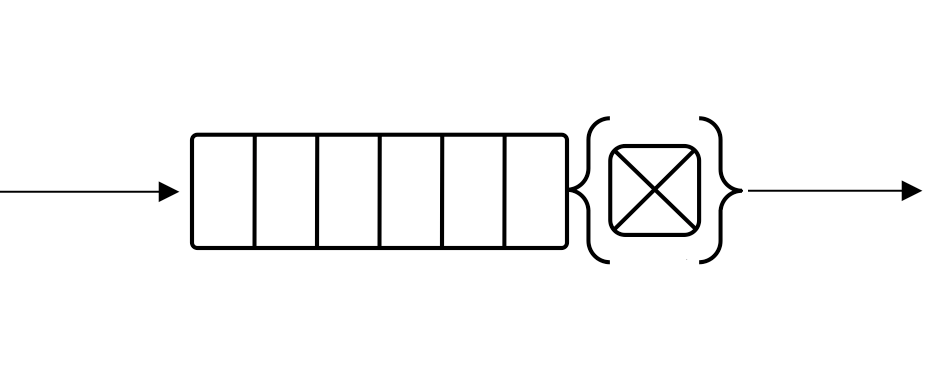
\includegraphics[width=0.45\textwidth]{Images/MM12.png}\qquad\qquad 
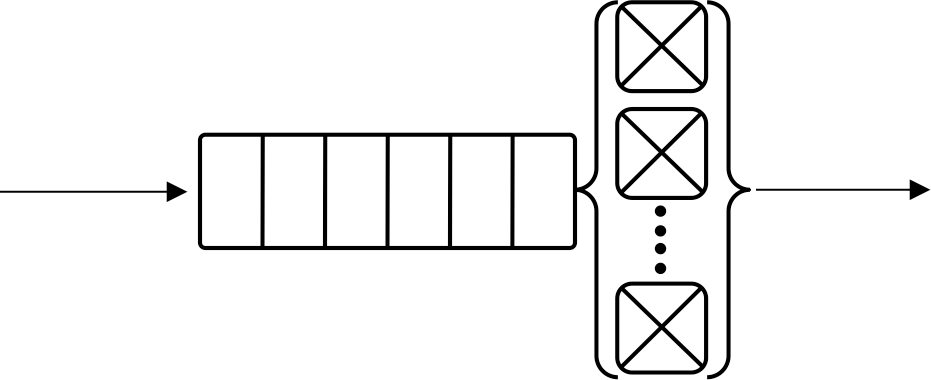
\includegraphics[width=0.45\textwidth]{Images/MMc.png}\\
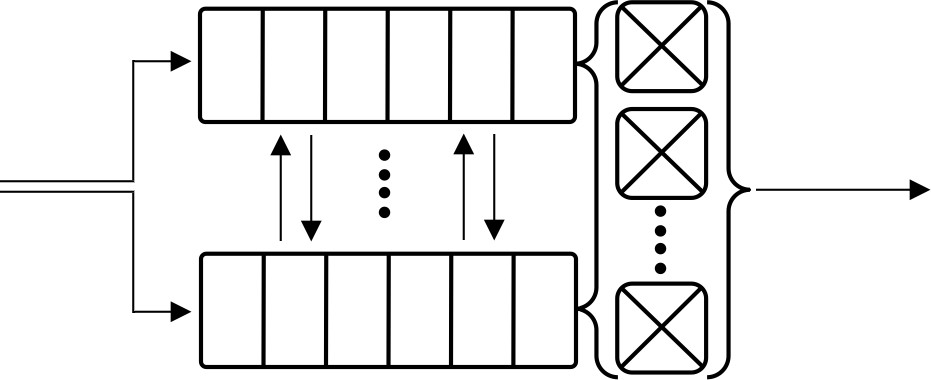
\includegraphics[width=0.45\textwidth]{Images/Tandem.png}
\caption{\small Schéma de systèmes de file d'attente ($M/M/1$, $M/M/c$, en tandem); les clients arrivent par la gauche, entrent dans la file d'attente, y demeurent jusqu'à ce qu'ils soient servis, puis sortent de la file.}\label{fig:MM}\hrule
\end{figure*}%\afterpage{\FloatBarrier}
$$
\pi_{0} = \left[1 + \frac{\left(c \rho\right)^{c}}{c! \left(1-\rho\right)} + \sum^{c-1}_{n=1} \frac{c \rho^{n}}{n!}\right]^{-1}\!\!. $$
Notons que, comme c'était le cas dans un système $M/M/1$, si $\rho \geq 1$, il ne peut y avoir d'état stable -- c'est-à-dire que si le taux d'arrivée est au moins aussi important que le taux de service maximum possible ($\lambda \geq c \mu$), le système ``explose''. \newl  Du point de vue du propriétaire, on peut vouloir s'assurer que les clients ne font pas la queue pendant un temps excessif, tout en réduisant au minimum le temps pendant lequel les serveurs restent en veille.  Dans un système $M/M/c$, la  probabilité que tous les guichets soient occupés (dans le régime stable) est donnée par 
$$ P( n \geq c) = \frac{\left(c \rho\right)^{c}}{c ! \left(1-\rho\right)} \pi_{0}.$$ 
Le tableau~\ref{tab:pns} donnent les valeur de $P( n \geq c)$ dans diverses situations.  
\begin{table}[!t]
\centering
\begin{tabular}{ccccccc}
\hline
$\rho$ & $c=2$ & $c=3$ & $c=4$ & $c=5$ & $c=6$ & $c=7$ \\
 \hline
.10& .02& .00& .00& .00& .00& .00 \\
.20& .07& .02& .00& .00& .00& .00 \\
.30& .14& .07& .04& .02& .01& .00 \\
.40& .23& .14& .09& .06& .04& .03 \\
.50& .33& .24& .17& .13& .10& .08 \\
.55& .39& .29& .23& .18& .14& .11 \\
.60& .45& .35& .29& .24& .20& .17 \\
.65& .51& .42& .35& .30& .26& .21 \\
.70& .57& .51& .43& .38& .34& .30 \\
.75& .64& .57& .51& .46& .42& .39 \\
.80& .71& .65& .60& .55& .52& .49 \\
.85& .78& .73& .69& .65& .62& .60 \\
.90& .85& .83& .79& .76& .74& .72 \\
.95& .92& .91& .89& .88& .87& .85 \\
\hline
\end{tabular}
\caption{\small Probabilités $P(n\geq c)$ que tous les serveurs/guichets soient occupés dans un système $M/M/c$ pour $c=2,\ldots, 7$ et $\rho\in (0.1,0.95)$ \cite[p.1088]{QS_W}.}\label{tab:pns}\hrule
\end{table}%\afterpage{\FloatBarrier}
On peut effectuer des calculs (assez difficiles, au demeurant) à l'aide de $W_{s} = \frac{1}{\mu}$, afin de montrer que $$ L_{q} = P( n \geq c) \frac{\rho}{1-\rho}, \ 
W_{q} = \frac{L_{q}}{\lambda}, \ 
W = \frac{1}{\mu} + W_{q}, \ 
 L = \frac{\lambda}{\mu} + L_{q}.$$ 
\begin{Exemple} Une banque a deux guichets. \`A chaque heure, 80 clients arrivent à la banque en moyenne et attendent dans une file unique qu'un guichet se libère. Supposons que le temps de service moyen est de 1.2 minute, et que les intervalles d'arrivée et les temps de service suivent des distributions enponentielles. Que sont:
\begin{itemize}[noitemsep]
	\item[(a)] le nombre prévu de clients dans la banque;
	\item[(b)] la durée prévue du séjour dans la banque pour le client moyen, et
	\item[(c)] la proportion du temps pendant laquelle les caissiers son inactifs.
\end{itemize}
\textbf{Solutions:} nous faison affaire à un système $M/M/2$ avec $\lambda =80 $ clients/h et $\mu = 50 $ clients/h. Ainsi, l'intensité de trafic est $\rho = \frac{80}{2\cdot 50} = 0.80 < 1$ et le système admet un régime stable. \begin{itemize}[noitemsep]
	\item[(a)] En consultant la table~\ref{tab:pns}, on constate que $$P(n \geq 2) = 0.71$$ pour $\rho=0.8$, d'où 
\begin{align*} L_{q} &= P( n \geq 2)\cdot \frac{.8}{1-.8} = 2.84 \text{ clients}\\
L& = 	\frac{80}{50} + L_{q}	= 4.44 \text{ clients.} \end{align*}
\item[(b)]	On a $W = \frac{L}{\lambda} = \frac{4.44}{80} = 0.055 \text{ hr }= 3.3 $ min.
\item[(c)] On détermine la proportion du temps pendant lequel un serveur est inactif en notant que les guichets sont inactifs à tout instant où $n=0 $, et la moitié du temps lorsque $n = 1$ (par symétrie) . La probabilité qu'un serveur reste inactif est donc donnée par $ \pi_{0} + 0,5 \pi_{1}$. Mais
 $$\pi_{0} = \left[1 + \frac{\left(2\cdot .8\right)^{2}}{2! \left(1-.8\right)} + \sum^{2-1}_{n=1} \frac{2\cdot .8^{n}}{n!}\right]^{-1}= \frac{1}{9}$$ et $$\pi_{1} = \frac{1.6}{1!} \pi_{0} = 0.176,$$ d'où la probabilité qu'un caissier spécifique est inactif est de $0.111 + 0.5(0.176) = 0.199$.
\end{itemize}
\end{Exemple}
\noindent \textbf{Remarque importante:} en général, les modèles de files d'attente ne sont pas compris dans la même mesure que le $M/M/1$ (et le $M/M/c$ dans une moindre mesure), et les mesures de performance ne sont souvent que des approximations fortement dépendantes des spécificités du problème en question. \par C'est pourquoi les modèles $M/M/c$ sont parfois utilisés même lorsque leur emploi n'est pas justifié par les données et observations (la situation n'est pas sans rappeler l'utilisation répandue de la distribution normale dans divers problèmes de probabilité et de statistiques). \par Dans de nombreuses applications, les distributions empiriques des arrivées et des temps de service approchent une distribution de Poisson et une distribution exponentielle, respectivement, de sorte que l'hypothèse n'est pas entièrement erronée, mais les simulations numériques ne devraient pas être évitées lorsque les écarts par rapport au modèle $M/M/c$ sont trop prononcés.